\section{System Design and Working Environment}
The hardware, labels, and interfaces in this section describe the physical system. The separate final simulation uses HSV detection, four red/blue cubes, two orange bridges, and MoveIt execution as detailed in Section~\ref{sec:simulation}; its topics and class mapping should not be substituted for the physical configuration.

\subsection{Hardware and communication}
The system has three main parts. The Windows computer starts the experiment and shows the camera preview. The Jetson runs the detector, the ROS 2 task controller, and the robot worker. The mechArm performs the joint movements and gripper actions. Keeping the decision and control programs on the Jetson avoids sending every small movement through the Windows preview connection.\src{defense,integration}

The supplied launcher connects to the Jetson at \file{192.168.55.1}. The worker reaches the arm through the TCP endpoint \file{192.168.100.2:9000}. These addresses describe the laboratory arrangement, rather than a general requirement of the algorithm. The camera image size used for region calibration is $1280\times720$ pixels.

\begin{figure}[H]\centering
\begin{tikzpicture}[font=\small,>=Latex,
 box/.style={draw=Navy,rounded corners=2pt,align=center,minimum height=1.15cm,text width=3.45cm,fill=PaleBlue},
 arr/.style={->,thick,color=Teal}]
\node[box] (win) {Windows computer\\Startup and live preview};
\node[box,right=0.65cm of win] (jet) {Jetson computer\\YOLO11 and ROS 2};
\node[box,right=0.65cm of jet] (arm) {mechArm 270\\Six joints and gripper};
\node[box,below=0.9cm of jet] (cam) {Fixed RGB camera\\Six source grids};
\draw[arr] (win) -- node[above,font=\scriptsize]{SSH} (jet);
\draw[arr] (jet) -- node[above,font=\scriptsize]{TCP} (arm);
\draw[arr] (cam) -- (jet);
\end{tikzpicture}
\caption{Hardware and communication structure. The drawing summarizes the deployment shown in the defense presentation.}
\label{fig:hardware}
\end{figure}

The real scene contains colored objects, marked cells, the gripper, and background items such as cables and a power adapter. Cables and the adapter sometimes resemble targets and were included in the background training examples. The real photographs used in this report come from the Experiment 3 slides.

\begin{figure}[H]\centering
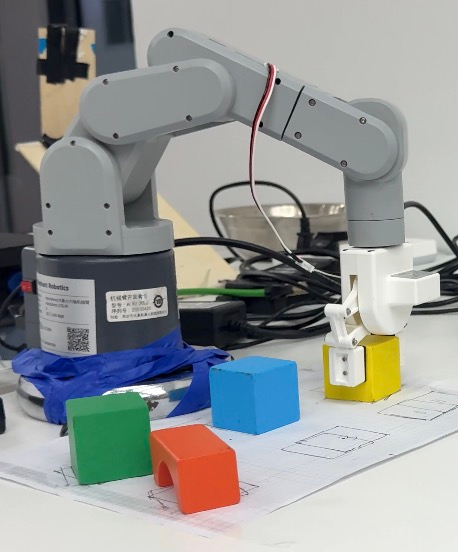
\includegraphics[height=6.0cm,keepaspectratio]{figures/robot_setup.png}
\caption{The mechArm and the tabletop objects in the supplied defense material, slide 7. The image shows the physical setup; it is not a measurement of position accuracy.}
\end{figure}

\subsection{Software modules and information flow}
The complete physical Launch file starts three ROS 2 nodes. The first node opens the camera, runs detection, publishes the raw image and detection array, and creates the preview and optional video. The second node maps detections to grids and runs the state machine. The third node receives one transfer request at a time and controls the arm.\src{integration,controller}

\begin{table}[H]\tabstart
\caption{Main software modules in the final physical pipeline}
\begin{tabularx}{\textwidth}{@{}L{5.75cm}Y@{}}
\toprule File or module & Main responsibility\\\midrule
\file{detector_node.py} & Camera input, YOLO boxes and labels, red/pink refinement, ROS publication, preview and video.\\
\file{experiment3_task_controller.py} & Grid assignment, stable group states, target selection, request tracking, timeout and task logs.\\
\file{experiment3_robot_worker.py} & Validate requests, run the transfer process, and return progress and completion feedback.\\
\file{experiment3_transfer_test.py} & Build the selected taught route, move the arm, check position and gripper feedback, and recover on errors.\\
\file{experiment3_region_}\newline\file{calibrator.py} & Create and check the six image polygons.\\
\file{experiment3_pose_recorder.py} & Record and save the named physical poses used by the six-grid task.\\
\bottomrule
\end{tabularx}
\end{table}

The image topic is \file{/camera/image_raw}, and the detection topic is \file{/yolo/detections}. A transfer request is sent on \file{/experiment3/transfer_requests}; worker responses return on \file{/experiment3/transfer_feedback}. The last two topics use JSON text inside ROS string messages. A request contains a request ID, grid ID, the detected six-class label after refinement, sorting group, destination, and detection confidence. The feedback links its status to the same request ID.

We use this request-and-feedback pair as the long-running task interface. It is implemented with topics rather than a ROS 2 Action server. The controller matches results by request ID and handles stale feedback and timeouts.

\subsection{Deployment, configuration, and module integration}
The supplied deployment process begins on Windows with configuration backup. The synchronization script downloads the active region polygons, gripper profiles, and 17-pose file from the original Jetson into the local package. This preserves the device settings before deployment. Changing the camera, robot base or gripper installation requires recalibration and pose checks.\src{integration,calibration,teaching}

The deployment script transfers the two ROS 2 packages, \file{yolo_detection_ros2} and \file{mecharm_pick_place}, into the Jetson workspace. It also uploads the hardware helpers, test scripts, model weights, and configuration files. On the Jetson, it sources ROS 2 Humble and runs \texttt{colcon build} with \file{--symlink-install} for these two packages. The startup script later sources both the ROS environment and the workspace installation, so ROS can find the built nodes.\src{integration}

The complete Launch file defines the active model, regions, poses, and gripper-profile paths in one place. The detector and controller receive the same region-file argument. This avoids displaying one set of grids while selecting actions from another. The active pose file and gripper profile belong to the same physical setup. 

The three node names are \file{experiment3_yolo_detector}, \file{experiment3_task_controller}, and \file{experiment3_robot_worker}. Their topic names provide fixed connections between modules. Windows opens an SSH tunnel from local port 18091 to Jetson preview port 8091, allowing the browser to show the remote image. The launcher checks for an existing robot controller and asks for one \texttt{RUN AUTO} entry before setting \file{armed:=true}. The Launch default is disarmed.\src{integration,controller}

Shutdown is also coordinated. Exit of the detector, controller, or worker triggers shutdown of the full Launch session. During cleanup, the worker attempts to stop an active runner, while the detector releases the camera and video resources. \src{integration,controller,vision}

A clear integration sequence is to check the connection and active files, build the packages, inspect the camera and grids in preview mode, and then check the taught routes and gripper settings through the dedicated tools. The complete run follows these module checks. Timestamped video and task logs then link visual decisions to requests and worker feedback.\src{integration,motion}

\subsection{Six labels and two destinations}
The detector retains six labels because the objects have different colors and shapes. The task controller reduces them to two movement groups. The distinction matters when a label is wrong. A blue-to-green cube error keeps the same destination. A pink-cube-to-red-cuboid error changes the destination.\src{vision,gripper}

\begin{table}[H]\tabstart
\caption{Class mapping and gripper targets}
\begin{tabularx}{\textwidth}{@{}L{4.7cm}C{1.6cm}C{2.3cm}Y@{}}
\toprule Detector label & Group & Destination & Closing target\\\midrule
\file{blue_cube} & cube & Right & 69\\
\file{green_cube} & cube & Right & 69\\
\file{pink_cube} & cube & Right & 69\\
\file{yellow_cube} & cube & Right & 69\\
\file{red_cuboid} & other & Left & 40\\
\file{orange_bridge} & other & Left & 40\\\bottomrule
\end{tabularx}
\end{table}

Both groups use an opening target of 100 and a gripper speed setting of 20. These values are device command values in the supplied profile. They are control values, not calibrated measurements of jaw angle or force. The profile is loaded from a configuration file so that a change in the gripper setup does not require rewriting the task logic.
